\section{Evolution of C}
\begin{figure}[hbtp]
\centering
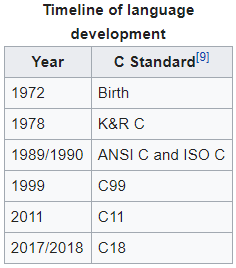
\includegraphics[width=200 px]{Source Images/Timeline of C language.png}
\caption{Evolution of C: Table Representation}
\end{figure}
C supports variable sized arrays from C99 standard.

\section{Array}
Here we will discuss about array data structure.\\
Reference: \href{https://www.geeksforgeeks.org/array-data-structure/}{GfG}\\

\subsection{Array rotation}
\subsection{Making subarray}
A subarray is a contiguous part of an array. An generated array that are already part of an another array.\\
e.g. : A given array - {1, 2, 3, 4}\\
Subarray of this array:
{1}, {2}, {3}, {4}, {1, 2}, {2, 3}, {3, 4}, {1, 2, 3}, {2, 3, 4}, {1, 2, 3, 4}
Given arrays are subarray of given array. A array holds $\frac{n(n+1)}{2}$ subarrays where $n$ is the number of elements in main array.

\section{Memory Allocation}
\subsection{Memory Layout of C}
Typical memory layout of C consists with following segments:-
\begin{enumerate}
	\item Text segment
	\item Initialized data segment
	\item Uninitialized data segment
	\item Stack
	\item Heap
\end{enumerate}
For better understanding, look at the block diagram below:-\\
\begin{figure}
	\centering
	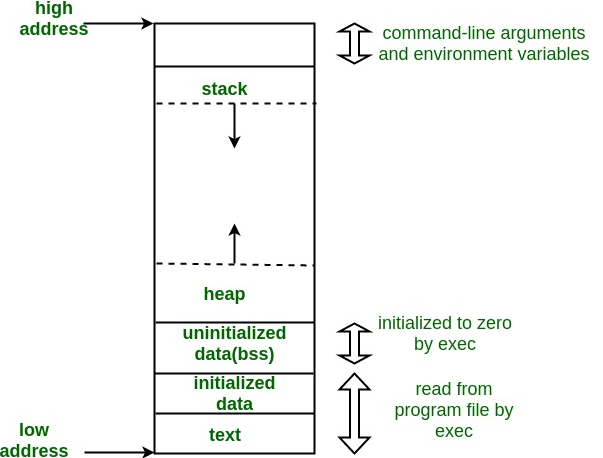
\includegraphics[width=200px, height=140px]{Source Images/C memory layout, GfG.png} 
	\caption{C memory layout, GfG}
\end{figure}
\pagebreak

\textbf{Short explanation:}
\begin{itemize}
	\item[$\rightarrow$] \textbf{A text segment}, known as code segment or simply text holder, is one of the section of a program that contains executable instructions as a text. As a memory region, a text segment may be placed below the heap or stack in order to prevent heaps and stack overflows from overwriting it.
	\item[$\rightarrow$] \textbf{Initialized data segment} usually called \textbf{Data Segment (\textcolor{red}{DS}}), is a portion of virtual address space of a program, which contains \textit{global variables} and \textit{static variables} that are initialized by the programmer.
	\item[$\rightarrow$] \textbf{Uninitialized data segment}, generally known as \textbf{\textcolor{red}{BSS}}, named after an ancient assembler operator that stood for "\textit{block started by symbol}". It contains all global variables and static variables that are initialized to zero or do not have explicit initialization in source code.
	\item[$\rightarrow$] \textbf{Stack} is the segment for storing non-static and local variables.
	\item[$\rightarrow$] \textbf{Heap} is the segment where dynamic memory allocation usually takes place. The heap area began at the end of the BSS segment and grows to larger addresses from there.
\end{itemize}
Wanna learn more?, follow the \href{https://www.geeksforgeeks.org/memory-layout-of-c-program/}{LINK}.

\subsection{Pointers}
\href{https://www.youtube.com/watch?v=f2i0CnUOniA&list=PLBlnK6fEyqRjoG6aJ4FvFU1tlXbjLBiOP&index=18&t=0s}{NESO Academy}\\
Pointers is a special type of variables which is capable to store initial address of a variable which is points to. That's mean, $x$ is a int variable and that takes byte in memory of the location at 1002 and 1003. Then a pointer that points $x$ will return 1002, the initial point.\\
General syntax for declaring pointer:-\\
\textcolor{red}{data\_type *pointer\_name;}\\
\begin{center}
	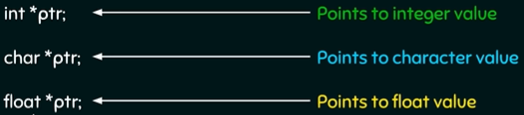
\includegraphics[width=180 pt]{Source Images/Pointer which is points to.png} 
\end{center}
We can assign values to the pointer by \textcolor{red}{address\_of} operator. Which is \textcolor{red}{Ampersand}.
\begin{center}
	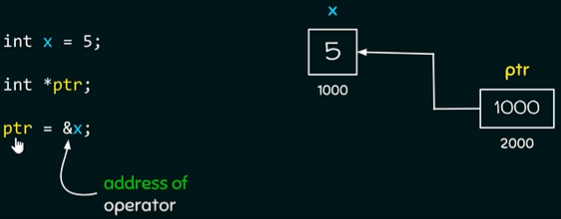
\includegraphics[width=180 pt]{Source Images/Assigning address to the pointer.png} 
\end{center}
We know that, pointer is also a variable so that it also takes place in memory and then store address of another variable in it.

\subsection{Dynamic Memory Allocation}
Dynamic memory allocation in C/C++ refers to performing allocate memory manually by the programmer. Dynamically allocated memories allocated on \textbf{HEAP}.\\
\begin{tcolorbox}
	Dynamic memory allocation is the process of assigning memory cell during execution time of the program.
		\begin{tcolorbox}[width=6.5cm, colframe=red!90]
			Run-Time memory allocation.
		\end{tcolorbox}
\end{tcolorbox}

\subsubsection{New and Delete operations}
Where C uses \textcolor{red}{malloc(}) function for dynamically allocate memory and free() for remove this. \textcolor{red}{malloc()} is a system function which allocates memory on the heap and returns a pointer to the new block. C++ standard supports these functions but also have two extra operator namely new and delete for performing same task in a better and easier way.\\
\textbf{New} is an operator which denotes a request to memory for allocate space on Heap. \textbf{New} operators initializes the memory and returns address of the newly allocated and initialized memory to the pointer variable.

\section{Illustration of C++ code}
 If there some problem with the STL of C++, then made own build in functions.
 Text before \dots
 \LaTeX
 \begin{lstlisting}
 for(int i=0; i<iterations; i++)
 {
  do something;
 }
 \end{lstlisting}
 Text after it \dots
 \subsection{Finding maximum element from an array of size n}

\begin{lstlisting}[frame=shadowbox, rulesepcolor=\color{blue!80}]
int MaxEle(int arr[], int n)
{
    int i, a=0;
    for(i=0; i<n; i++)
    {
        a = max(a, arr[i]);
    }
    return a;
} 
\end{lstlisting}

\subsection{Counting selected element from an array}
 
\begin{lstlisting}[frame=shadowbox, rulesepcolor=\color{green!80}]
int Count(int arr[], int n, int value)
{
    int c=0, i;
    for(i=0; i<n; i++)
    {
        if(arr[i]==value)
        {
            c++;
        }
    }
    return c;
}
 \end{lstlisting}
 
\subsection{Divide function by string}

\begin{tcolorbox}
\begin{lstlisting}
#include <bits/stdc++.h>
using namespace std;

string divide(string &ns, int &dividor, int &rem)
{
    int i;
    string result;
    rem = ns[0] - '0';
    for (i = 1; i < ns.size(); i++)
    {
        if (rem < dividor)
        {
            rem = rem * 10 + (ns[i] - '0');
            i++;
        }
        result.push_back(rem / dividor + '0');
        rem %= dividor;
    }
    return result;
}

int main()
{
    string ns;
    int dividor, rem;
    rem = 0;
    cin >> ns >> dividor;
    cout << ns << "/" << dividor << " = "
         << divide(ns, dividor, rem) << endl;
    cout << "Reminder: " << rem << endl;
}
\end{lstlisting}
\end{tcolorbox}

\subsection{BitWise Operator}
Works at bit-level.
Do we know that? Every odd number in binary representation hold true bit in first and last bit.
\begin{table}
\caption{Odd numbers in binary}
 \begin{center}
  \begin{tabular}{c c}
  ODD Decimal & in Binary\\
  1 & 1\\
  3 & 11\\
  5 & 101\\
  7 & 111\\
  9 & 1001 
  \end{tabular}
 \end{center}
\end{table}
Is it clear? OK. As reverse way, all even number in binary representation hold first true bit and false in last. For the sake of illustration:-
\begin{table}
\caption{Even numbers in binary}
 \begin{center}
  \begin{tabular}{c c}
  EVEN Decimal & in Binary\\
  2 & 10\\
  4 & 100\\
  6 & 110\\
  8 & 1000\\
  10 & 1010 
  \end{tabular}
 \end{center}
\end{table}

Bitwise operators works on binary bits of given number.
\subsubsection{Some Interesting things about bitwise operator}
\begin{enumerate}
 \item 'N' is a given number, N will be odd if bitwise operation between N and 1 is 1. Means: (N\&1)=1, if N if odd. Else 0 if N is even.
 \item The left shift and right shift operators should not be used for negative numbers.
 \item We can find odd occurring number in an array by XOR.\\
 \begin{lstlisting}
 s;kldf
 \end{lstlisting}
\end{enumerate}

\subsection{Structure}
\begin{lstlisting}[basicstyle=\footnotesize, frame=single, frameround=tftf, numbers=left, stepnumber=2, numberfirstline=false, caption=Structure in C/C++]
#include<bits/stdc++.h>
using namespace std;

///Now we gonna learning structure in C++.
/*
    Sometimes we need a group of different types
    data in one specific class collection. For get
    released from this problem, C and C++ provides
    a new user-defined data-type.
    To define a structure, use the keyword "struct".
*/
struct student
{
    /*
        All members of struct is generally public.
    */
    int ID;
    string sex;
};

int main()
{
    /*
        Let's declare a student struct of class 6 that
        has 3 students.
        First student(class6[0]) has 33 as roll.
    */
    student class6[3];
    class6[0].ID=33;
    class6[1].ID=34;
    cout << class6[0].ID << endl;
    cout << class6[1].ID << endl;
    student kiron;
    cin >> kiron.ID;
    cout << "Kirons id " << kiron.ID << endl;
    cin >> kiron.sex;
    cout << "Kirons sex " << kiron.sex << endl;

    /*
        Let's declare a pointer of type student.
        That can store address of student type variables.
    */
    student *ptr;
    /*
        Now This pointer will store address of kiron's all
        member function.
    */
    ptr = &kiron;
    /*
        Now ptr points to all member variable of
        struct variable kiron.
    */

    kiron.ID=65;
    ptr->sex="Male";
    cout << ptr->ID << endl;
    cout << kiron.sex << endl;
    /*
    	Arrow operator is used for access by pointer.
    */
}
\end{lstlisting}

\subsection{How to check efficiently that a number is palindrome or not}
\href{https://leetcode.com/articles/palindrome-number/}{Link}\\
\begin{flushleft}
\textbf{Intuition}
The first idea that comes to mind is to convert the number into string, and check if the string is a palindrome, but this would require extra non-constant space for creating the string which is not allowed by the problem description.\linebreak
\linebreak
Second idea would be reverting the number itself, and then compare the number with original number, if they are the same, then the number is a palindrome. However, if the reversed number is larger than \textbf{int.MAX}, we will hit integer overflow problem.
\linebreak
\linebreak
Following the thoughts based on the second idea, to avoid the overflow issue of the reverted number, what if we only revert half of the \textbf{int} number? After all, the reverse of the last half of the palindrome should be the same as the first half of the number, if the number is a palindrome.
\linebreak
\linebreak
For example, if the input is 1221, if we can revert the last part of the number "1221" from "21" to "12", and compare it with the first half of the number "12", since 12 is the same as 12, we know that the number is a palindrome.
\end{flushleft}
\textbf{Algorithm}\\
First of all we should take care of some edge cases. All negative numbers are not palindrome, for example: -123 is not a palindrome since the '-' does not equal to '3'. So we can return false for all negative numbers.
\linebreak
\linebreak
Now let's think about how to revert the last half of the number. For number 1221, if we do 1221 \% 10, we get the last digit 1, to get the second to the last digit, we need to remove the last digit from 1221, we could do so by dividing it by 10, 1221 / 10 = 122. Then we can get the last digit again by doing a modulus by 10, 122 \% 10 = 2, and if we multiply the last digit by 10 and add the second last digit, 1 * 10 + 2 = 12, it gives us the reverted number we want. Continuing this process would give us the reverted number with more digits.
\linebreak
\linebreak
Now the question is, \textit{how do we know that we've reached the half of the number?}
\linebreak
\linebreak
Since we divided the number by 10, and multiplied the reversed number by 10, when the original number is less than the reversed number, it means we've processed half of the number digits.

 \section{STL Map}
 Map is a associated container of C++ STL(Standard Template Library). A map variable has two part,
 
 \begin{enumerate}
  \item Key
  \item Value
 \end{enumerate}
 
 \href{https://www.geeksforgeeks.org/map-associative-containers-the-c-standard-template-library-stl/}{\textcolor{blue}{Geeks for Geeks}}: Maps are associative container that stores data in a mapped fashion. No two map values can have same key values.\\
 
 \begin{lstlisting}
  #include<map>
  // Declaring Map
  map<int, int> mp; // mp: map name.
  // First one is keyvalue, second one is mapvalue.
  
  // Insert elements in random order.
  mp.insert(pair<int, int>(1, 40));
  
  //Creating map iterator:
  map<int, int> :: iterator it;
  
  //Accessing the map data:
  it -> first; // Refer keyvalue.
  it -> second; // Refer mapvalue.
 \end{lstlisting}
 
  \subsection{Map member function}
   1. insert() :- The key must be unique.
   
   \begin{lstlisting}
   //Syntax:
    map_name.insert({key, value});
    
    //e.g.
    map<int, int> mp;
    mp.insert({1, 40});
   \end{lstlisting}
   
   2. count() :-
      
   \section{STL pair}
   
   \begin{lstlisting}
#include<iostream>

/*For pair access, include this header file.
utility is a STL.*/
#include<utility>
using namespace std;

int main()
{
    pair<int, int>p1;
    p1.first = 1;
    p1.second = 2;
    cout << p1.first << " " << p1.second << endl;

    ///Declaring pair array with the size 4.
    pair<int, int>p[4];
    //All pair value assigned to 0 automatically.

    p[0].first=1;
    p[0].second=2;
    cout << p[0].first << " " << p[0].second << endl;

    /*Here we not assigned any value to the pair p[1] and p[2].
    So there will print 0*/
    cout << p[1].first << " " << p[1].second << endl;
    cout << p[2].first << " " << p[2].second << endl;

    /*
     Member function: make_pair().
     This member function assign values to pair directly.
     Thats mean, this is more sexy.
     Syntax: pair_name = make_pair(value1, value2);
    */
    pair<string, double> ps;
    ps = make_pair("My S.S.C result: ", 4.56);
    cout << ps.first << ps.second << endl;

    /*
     Operating pairs.
     1. (==) comparison.
        It will return 1 is those pairs both values are equal otherwise 0.
        As same for all other comparisons like >=, <=, != etc.
    */
    pair<int, int> pair1, pair2, pair3;
    pair1 = make_pair(1, 4);
    pair2 = make_pair(1, 4);
    pair3 = make_pair(2, 4.1);
    /*No matter what type value we assigned,
    It will type casted automatically by the data type as we declared.
    So it will be same as (2, 4).
    */

    if(pair1==pair2)
    {
        cout << "Pairs are same" << endl;
    }
    cout << (pair1==pair2) << endl;
    if(pair1!=pair3)
    {
        cout << "pair1 and pair3 are not same" << endl;
    }
    else
    {
        cout << "pair1 and pair3 are same" << endl;
    }

    /*
     swap()
     Syntax: pair1.swap(pair2);
     It will swap values of both pair.
     swap pair1.first with pair2.first then
     swap pair1.second with pair2.second
    */
    pair1.swap(pair3);
    cout << pair1.first << " " << pair1.second << endl;
    
    /*
     swap() isn't working in code::blocks but in other
     online compiler, it works perfectly.
     */
}


   \end{lstlisting}
   
\section{STL List}
Lists are sequence of elements stored in a linked list. Compared to vectors, they allow fast insertions and deletions, but slower random access.\\
\subsection{Member Functions of List}
\begin{tabular}{|c c|}
\hline
Function & Task\\
\hline
assign & assign elements to list\\
\hline
begin & returns an iterator to the beginning of the list\\
\hline
back & returns a reference to last element of list\\
\hline
clear & removes all elements from the list(Clears the list)\\
\hline
empty & returns true if list is empty\\
\hline
end & returns an iterator just past the last element of a list\\
\hline
erase & remove specific element from list\\
\hline
front & returns a reference to the first element of a list\\
\hline
insert & insert elements into the list\\
\hline
max\_size & returns the maximum number of elements that the list can hold\\
\hline
merge & merge two lists\\
\hline
push\_back & add an element at end of the list\\
\hline
push\_front & add an element at beginning of the list\\
\hline
pop\_back & removes the last element of the list\\
\hline
pop\_front & remove first element of the list\\
\hline
rbegin & return reverse begin iterator\\
\hline
rend & return reverse end iterator\\
\hline
remove & remove elements from list\\
\hline
remove\_if & remove element conditionally\\
\hline
resize & change size of the list\\
\hline
reverse & reverse the list\\
\hline
size & returns the numbers of elements present in the list\\
\hline
sort & sorts the list in ascending order\\
\hline
splice & merge the lists in constant time\\
\hline
swap & swap two list with each other with all elements\\
\hline
\textcolor{red}{unique} & removes duplicate element\\
\hline
\end{tabular}
\subsection{Discuss}
\begin{lstlisting}
vector<int> v(5, 42);
\end{lstlisting}
It will produce a vector named v with five times 42.\\
\begin{lstlisting}[frame=shadowbox, rulesepcolor=\color{green!60}]
#include<bits/stdc++.h>
using namespace std;

int main()
{
    vector<int> v(5, 42);
    for(int i=0; i<v.size(); i++)
    {
        cout << v[i] << " ";
    }
    cout << endl;
}
\end{lstlisting}
\begin{tcolorbox}[colback=black!3]{Output:}
42 42 42 42 42
\end{tcolorbox}
\subsection{assign}
assign member function is used assign values from one to another.\\
\begin{lstlisting}[frame=shadowbox, rulesepcolor=\color{green!60}]
#include<bits/stdc++.h>
using namespace std;

int main()
{
    vector<int> v1;
    for(int i=0; i<10; i++)
    {
        v1.push_back(i);
    }
    vector<int> v2;
    v2.assign(v1.begin(), v1.end());
    for(int i=0; i<v2.size(); i++)
    {
        cout << v2[i] << " ";
    }
    cout << endl;
}
\end{lstlisting}

\section{STL Stack}
\begin{lstlisting}[caption=Stack, frame=shadowbox, rulesepcolor=\color{green!70}]
#include<iostream>
#include<stack>
using namespace std;

/*
 Stacks are a type of container adaptors with LIFO(Last IN First Out).
 So we can say, stack is Stup.
*/

int main()
{
    /*Let's create a stack of int type.*/
    stack<int> s;

    /*Member function push() will add the new element at the top
    of the stack.
    Time complexity O(1)*/
    s.push(10);
    s.push(9); /*9 stored above of 10*/
    s.push(8);
    s.push(1); /*Now 1 is the top most element.*/

    /*Algorithmic function size() returns current size of
    this stack.*/
    cout << s.size() << endl;

    /*Member function top() will return topper element or that element
    we entered last.
    For this example, it is 1*/
    cout << s.top() << endl;

    /*Member function pop() will delete the topmost element.*/
    s.pop();
    
    /*After removing topmost element,
    present topmost element is 8*/
    cout << s.top() << endl;
    
    /*After removing one element,
    current size of stack is 3*/
    cout << s.size() << endl;

    /*Algorithmic function empty() will return true if there is
    no element at the stack.*/
    if(!s.empty())
    {
        cout << "Stack is not empty" << endl;
    }

    return 0;
}
\end{lstlisting}
\begin{center}
\begin{tcolorbox}[enhanced, title=Output,
attach boxed title to bottom center, width=3.9 cm]
4\\1\\8\\3\\Stack is not empty
\end{tcolorbox}
\end{center}
   
\section{Power of 2}
\subsection{Binary Transform of \textbf{$2^n$}}
Look at the table:-\\(\LaTeX  provides a large set of tool for formatting tables)\\

\begin{center}
\begin{tabular}{||c | c | c | c||}
\hline
$2^n$ & Decimal & Binary & Seems like\\
\hline\hline
$2^0$ & 1 & 1 & $10^0$\\
\hline
$2^1$ & 2 & 10 & $10^1$\\
\hline
$2^2$ & 4 & 100 & $10^2$\\
\hline
$2^3$ & 8 & 1000 & $10^3$\\
\hline
$2^4$ & 16 & 10000 & $10^4$\\
\hline
$2^5$ & 32 & 100000 & $10^5$\\
\hline
\end{tabular}
\end{center}

It's clear that power of 2 in binary holds just one and only one true bit. So, we can simply say that, a number will be power of 2 if its binary holds just one true bit at first.

\subsection{Algorithm}
\begin{tcolorbox}
\begin{enumerate}
\item Take a decimal number string "ds".
\item Convert the number into binary string by a function.
 \begin{enumerate}
 \item Return binary string name such as "bs".
 \end{enumerate}
\item Start checking from the index 1.
\item If find out a true bit
 \begin{tcolorbox}
 return false;
 \end{tcolorbox}
 That mean, this is not power of 2.
\item Else: Till to end, there is no true bit.
 \begin{tcolorbox}
 return true;
 \end{tcolorbox}
 That mean, this is power of 2.
\end{enumerate}
\end{tcolorbox}

\section{Linked Lists}
Reference: \href{https://www.youtube.com/watch?v=njTh_OwMljA}{\textcolor{red}{Hacker Rank}}\\
Today we are going talk about linked lists. It's essentially just a sequence of the element, where each element links to the next elements which next element links to the next elements. A linked list can contain pretty much any kind of data - string, char, int. The elements can be sorted or unsorted, duplicates or unique. If we want to access element from linked list, we need linear time where array give us constant time, because for access array element, just boom, instantly do that. There are two type of linked list. Singly linked list and doubly linked list. Doubly linked list is a alternate version of singly linked list and access of elements from doubly link list is pretty much easy. One doubly linked list element has two part. One is previous node a second is next element. That mean, each elements having a link to the next element, each elements also linked to the previous element. So, for certain operations, this can be quite handy.\\
\href{https://www.geeksforgeeks.org/linked-list-set-1-introduction/}{\textcolor{red}{Geeks for Geeks}}\\
Advantages over arrays:-
\begin{itemize}
	\item Dynamic size
	\item Ease of insertion and deletion
\end{itemize}
Drawbacks:-
\begin{enumerate}
	\item Random access not allowed. We have to access elements sequentially from the first node called HEAD. So we can't do binary search with linked lists efficiently with its default implementation.
	\item Extra memory allocation required for a pointer with each elements of the list.
	\item As array, elements are not stored in contiguous location.
\end{enumerate}
Representation:-\\
A linked list is represented by a pointer to the first node of the linked list. If the linked list is empty, then the value of the HEAD is NULL. A node consist with two parts:-
\begin{itemize}
	\item Data
	\item Reference to the next node, i.e. pointer*.\footnote{\texttt{\hspace{0.4 cm}*A pointer is a special type of variable that stores memory address of another variable. Pointer is declared by asterisk sign before which variable we want to declare that it is a pointer. We can access address of a variable by using ampersand sign before it.}}
\end{itemize}

Let's create a user-defined data-type for build a node. A node has two part, one data and another pointer that points to the next node(That also has two part). So, the pointer must be such type that holds the next node(with two part). Means the pointer must be a node object.
IN C, node represented by struct. IN object-oriented language, it does with Class. Here the implementation in C++.
\begin{lstlisting}[caption=Node Class]
	class Node
	{
	 public:
	 	int data;
	 	Node *next;
	};
\end{lstlisting}
Block illustration of this code:-\\
\tikz
{
	\draw (0, 0)--(1, 0)--(1, -0.5)--(0, -0.5)--(0, 0);
	\draw (0.5, 0)--(0.5, -0.5);
	\draw[->] (1, -0.25)--(1.5, -0.25);
	\draw (1.5, 0)--(2.5, 0)--(2.5, -0.5)--(1.5, -0.5)--(1.5, 0);
	\draw (2, 0)--(2, -0.5);
	\draw[->] (2.5, -0.25)--(3, -0.25);
	\draw (3, 0)--(4, 0)--(4, -0.5)--(3, -0.5)--(3, 0);
	\draw (3.5, 0)--(3.5, -0.5);
}

 \section{Fortran}
 \textbf{Fortran} means Formula Translation. This is a general-purpose, compiled imperative programming language that's are specially suited to numeric computation and scientific computing, originally developed by IBM.\\
 (\textbf{IBM} - \textit{International Business Machines Corporation.})

\section{Python}
 In Linux and Mac operating systems, python are already installed. For install in windows, first we need to go \href{https://www.python.org/}{\textcolor{blue}{Pythons Official Website}}. Then download python and install.\\
\subsection{Why we use Python}
 Easy to learn, easy to use
 Popular in web development
 Can create a full web application